\chapter{Pug.js}

Pug.js (abbreviated as Pug) files are translated into HTML files, they provide the basic structure of the web page. Now let's learn how to write our own web page using Pug.

\section{Further Resources (Ch 5)}

I didn't have this piece of notes back when I first learned Pug. Here is \href{https://youtu.be/kt3cEjjkCZA}{the video}\footnote{Link: \url{https://youtu.be/kt3cEjjkCZA}{the video}} that I used to learn the basics. 

You could refer to the \href{https://www.w3schools.com/tags/default.asp}{w3schools documentation}\footnote{Link: \url{https://www.w3schools.com/tags/default.asp}} to learn how to use some more HTML tags.

\section{Magic on the Pug.js website}

The \href{{https://pugjs.org/}}{Pug.js official website}\footnote{Link: \url{https://pugjs.org/}} contains a detailed documentation on how it is translated to HTML.

What's more valuable is its interactive translator, you can just type any Pug code on any page in the documentation, \href{https://pugjs.org/language/attributes.html}{like this one}\footnote{Link: \url{https://pugjs.org/language/attributes.html}}, type Pug code on the left box and it will translate to HTML code on the right. It is a very useful tool to experiment with the Pug language.

\begin{figure}[h]
\centering
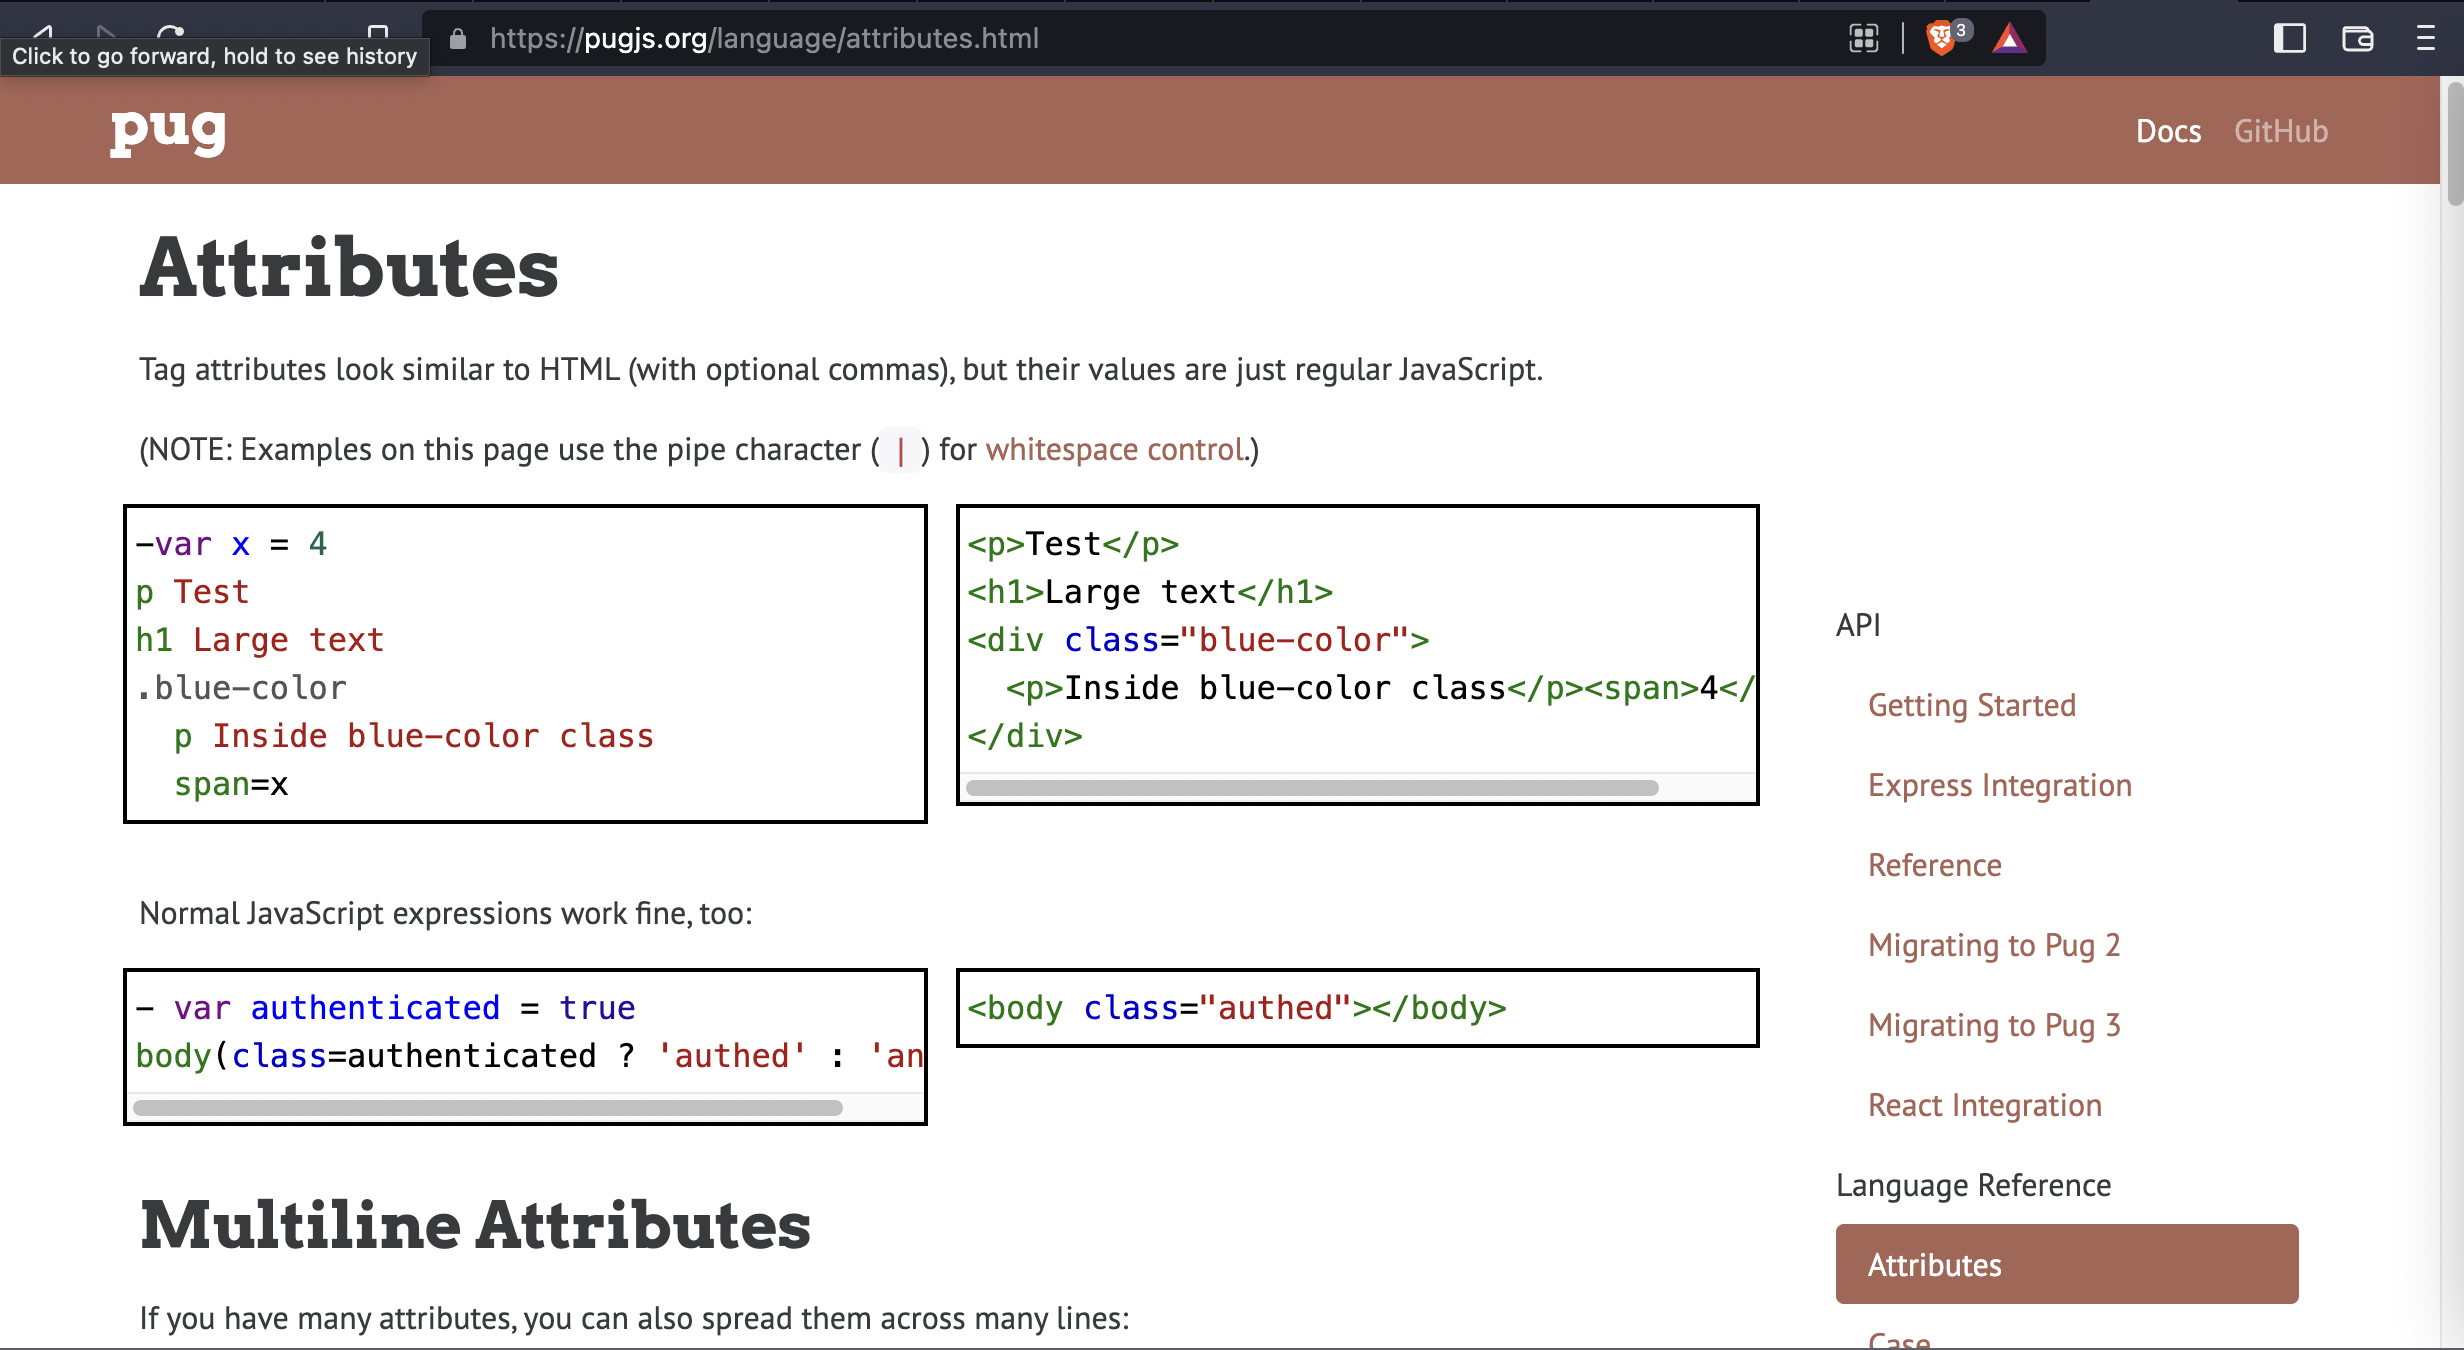
\includegraphics[width=13cm]{images/ch5-puginteractive.png}
\caption{Example usage of the interactive translator on the Pug.js official website}
\end{figure}

\section{HTML Tags}

Some of you haven't coded in HTML before, so here is a quick walkthrough to the basics of HTML, but using Pug.js syntax. For those of you who have used HTML before, mind the syntactical difference, a summary of the differences will be provided in one of the \hyperref[sec:pugvshtml]{sections below}. You can experiment the output in any file under \texttt{app/templates/views}, under the \texttt{block content} section.

\subsection{Normal text}

\texttt{p} stands for paragraph. Use this for normal text.
\vspace{6mm}

\begin{lstlisting}[language=pug]
p Hello world
\end{lstlisting}

\subsection{Headers}

\texttt{h1} stands for header 1, \texttt{h2} stands for header 2, and so on until \texttt{h6}. With \texttt{h1} being the largest. Use this for titles and subheadings.
\vspace{6mm}

\begin{lstlisting}[language=pug]
h1 header 1
h2 header 2
h3 header 3
h4 header 4
h5 header 5
h6 header 6
\end{lstlisting}

\subsection{Images}

\texttt{img} stands for image. You need to specify the source \texttt{src} of the image using \textbf{attributes}, we surround the attributes in parenthesis in Pug. Please make sure you add your images in the \texttt{app/images} folder.
\vspace{6mm}

\begin{lstlisting}[language=pug]
img(src="images/pi-green.png")
\end{lstlisting}

You can specify its width and height in pixels.

\begin{lstlisting}[language=pug]
img(src="images/pi-green.png" width=100 height=100)
\end{lstlisting}

\subsection{Links}

Use the \texttt{a} tag for links. It requires an \texttt{href} attribute indicating where the link should go.
\vspace{6mm}

\begin{lstlisting}[language=pug]
a(href="abouts.html") Click to go to the abouts page.
\end{lstlisting}

To open a brand new tab instead of replacing the current one, add the attribute \texttt{target = "\textunderscore blank"}
\vspace{6mm}

\begin{lstlisting}[language=pug]
a(href="https://www.google.com" target="_blank") Click to open Google on a new tab.
\end{lstlisting}

\subsection{Lists}

We surround all contents of a list within a \texttt{ul} or a \texttt{ol} tag. We use \texttt{ul} (unordered list) when we need bullet points, while we use \texttt{ol} (ordered list) when we need numbering. Each bullet point is demoted by \texttt{li} (list element).

The "surrounding" I mentioned is achieved by indenting all \texttt{li} tags within the \texttt{ul} or \texttt{ol} tags.
\vspace{6mm}

\begin{lstlisting}[language=pug]
ul
    li Apples
    li Oranges
    li Pears

p When you got an error message you should:
ol
    li Copy the error message
    li Go to <a href="https://www.google.com"> Google</a>
    //- The syntax used for the a tag will be discussed in the br tag section.
    li Paste and search for the error message
    li Click on the first stack overflow result
    li Copy and paste the solution
\end{lstlisting}

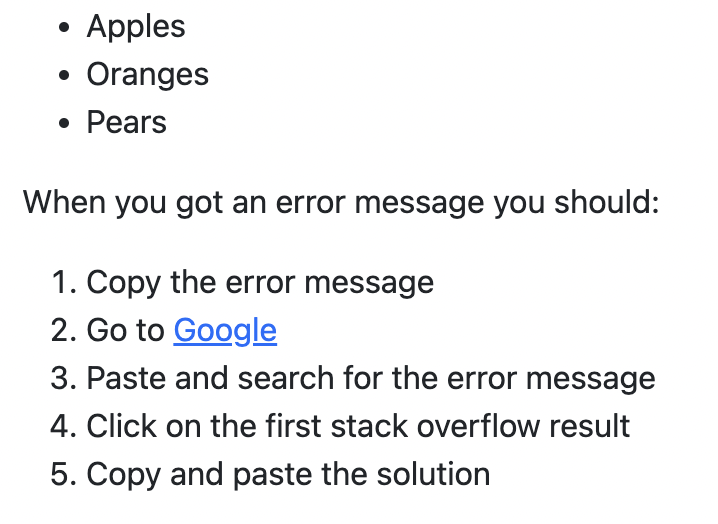
\includegraphics[width=10cm]{images/ch5-ulol.png}

\subsection{\texttt{div}}

\texttt{div} stands for divider. It serves no purposes in adding content to the web page, but it can be used to improve organisation of your code, and it is crucial for styling. We will discuss more in the \hyperref[sec:classesids]{next section} and also in the \hyperref[sec:ch6]{next chapter}.
\vspace{6mm}

\begin{lstlisting}[language=pug]
div
    h1 Self introduction
    p ...
div
    h1 Contact methods
    ul
        li ...
        ...
\end{lstlisting}

\subsection{\texttt{br}}

When the text is too long, you can put a \texttt{.} after the tag, and it now regards what indented within the tag as text.

\begin{lstlisting}[language=pug]
p.
    Hello, I am KidProf.
    I am a university student studying Computer Science.
    I like coding.
\end{lstlisting}


\includegraphics[width=15cm]{images/ch5-textinaline.png}

But when you look at the output, they are all on the same line. This is because the line breaks you made in the code is independent of the line breaks shown on the web page, you need to explicitly use \texttt{br} tags for line breaks. Because we are inside the \texttt{p} tag, Pug regards everything inside as text but not tags, but we can still use conventional HTML syntax to get around it.

\begin{lstlisting}[language=pug]
p.
	Hello, I am KidProf. <br />
	I am a university student studying <br />Computer Science.<br />
	I like coding.
\end{lstlisting}


\includegraphics[width=15cm]{images/ch5-textmultiplelines.png}

Alternatively, if you do not like that normal HTML code in your Pug code, you could do this instead and lead to the same result. But this is a lot of effort and affects code readability.

\begin{lstlisting}[language=pug]
p
	| Hello, I am KidProf.
	br
	| I am a university student studying
	br
	| Computer Science.
	br
	| I like coding.
\end{lstlisting}

The removal of the \texttt{.} after \texttt{p} indicates that what indented within are tags instead of plain text, so the \texttt{br} tags are registered. To indicate that the rest are plain text, the \texttt{|} character is used.

\subsection{Comments}

Use \texttt{//-} for comments.\footnote{An alternative is \texttt{//}, using \texttt{//} means that the generated HTML file would also contain that comment, while using \texttt{//-} won't.}

\subsection{I am lazy}
There are also other useful HTML tags, like \texttt{table}, \texttt{tr}, \texttt{td}, \texttt{span}, \texttt{small}, \texttt{button}, \texttt{input}. You could refer to the \href{https://www.w3schools.com/tags/default.asp}{w3schools documentation}\footnote{Link: \url{https://www.w3schools.com/tags/default.asp}} to learn how to use these tags. The translation to Pug is similar to the tags mentioned above.

\section{Classes and IDs}
\label{sec:classesids}

We need the notion of classes and IDs to do styling in the \hyperref[sec:ch6]{next chapter}, so that we can reference elements that we would like to style from the styling files.

We use \texttt{\#} followed by text to indicate an ID, and we use \texttt{.} followed by text to indicate a class. ID and class names must not contain spaces, it is a convention to either use camelCase or hyphens in place of spaces.
\vspace{6mm}

\begin{lstlisting}[language=pug]
div#self-intro
	h1 Self introduction
	p.large-text.
		Hello, I am KidProf. <br />
		I am a university student studying <br />Computer Science.<br />
		I like coding.
ul#shopping-list
	li Apples
	li.warning Oranges
	li.warning Pears
p When you got an error message you should:
ol#error-list
	li Copy the error message
	li Go to <a href="https://www.google.com"> Google</a>
	li Paste and search for the error message
	li Click on the first stack overflow result
	li Copy and paste the solution
a(href="#self-intro") Back to top
\end{lstlisting}

In the code above we have defined a few IDs, including \texttt{\#self-intro}, \texttt{\#shopping-list}, \texttt{\#error-list}; and also a few classes, including \texttt{.warning} and \texttt{.large-text}. 
\vspace{6mm}

\textbf{IDs must be unique within a page, while there can be multiple elements with the same class name in the same page.} An element can have more than one class.
\vspace{6mm}

To demonstrate one of the uses of IDs, I have included a link at the bottom of the example code. When you click on it, it brings you to the start of the page, to the element with ID \texttt{self-intro}. This feature does not work for classes because multiple elements can have the same class name in the same page.

The use of classes and IDs would become clearer in the \hyperref[sec:ch6]{next chapter}.

\section{Pug VS HTML syntax}
\label{sec:pugvshtml}

\textit{Skip if you have not learnt HTML before, this section aims to allow HTML programmers to relate what we are learning to what they have learnt}
\vspace{6mm}

Pug uses indentation to indicate that something is in a tag while HTML uses closing tags.
\vspace{6mm}

\begin{lstlisting}[language=pug]
//- pug
ul
  li A
  li B
  li C
\end{lstlisting}

\begin{lstlisting}[language=html]
<!-- HTML - poorly formatted, but would still work! -->
<ul><li>A</li><li>B</li><li>C</li></ul>
\end{lstlisting}

All attributes should be put within parenthesis after the tag in Pug, while attributes should be put within the opening tag in HTML.
\vspace{6mm}

\begin{lstlisting}[language=pug]
//- pug
a(href="abouts.html") Click to go to the abouts page.
\end{lstlisting}

\begin{lstlisting}[language=html]
<!-- HTML -->
<a href="abouts.html">Click to go to the abouts page.</a>
\end{lstlisting}

Classes and IDs declarations can be simplified with Pug using the syntax shown in the \hyperref[sec:classesids]{last section}.
\vspace{6mm}

\begin{lstlisting}[language=pug]
//- pug
a#abouts-link.class1.class2(href="abouts.html") Click to go to the abouts page.
\end{lstlisting}

\begin{lstlisting}[language=html]
<!-- HTML -->
<a href="abouts.html" id="abouts-link" class="class1 class2">Click to go to the abouts page.</a>
\end{lstlisting}

